%%%%%%%%%%%%%%%%%%%%%%%%
% RESIDUAL CALIBRATION %
%%%%%%%%%%%%%%%%%%%%%%%%
There are situations where the strong assumption of known residual variances \(\bm{\Sigma}_i = \sigma_i^2 \bm{I}_3\) is somewhat restrictive.
Thus we generalize multilevel inversion as in \cref{sec:PEM:CaseStudies:ProbInv} by treating \(\sigma_{\mathcal{E}} \equiv \sigma_i\) as a global unknown.
% PRIOR MODEL
In units of \(\unit[]{mm}\) the corresponding parametric prior is set to a uniform distribution \(\pi(\sigma_{\mathcal{E}}) = \mathcal{U}(0,0.5)\).
% EXPERIMENTAL SETUP
Otherwise the experimental setup of probabilistic inversion is used.
\par % INFERENTIAL MECHANISM
The standard deviation \(\sigma_{\mathcal{E}}\) of the residual model \(\mathcal{N}(\bm{\varepsilon}_i \cond \bm{0},\sigma_{\mathcal{E}}^2 \bm{I}_3)\)
is introduced as an extra unknown in the model \cref{eq:PEM:ProbInv:Model} and in the posterior \cref{eq:PEM:ProbInv:JointPosterior}.
% PRIOR & POSTERIOR
Consequently the joint prior is given as \(\pi(\tuple{E_i},\mu_E,\sigma_E,\sigma_{\mathcal{E}}) = \pi(\sigma_{\mathcal{E}}) \, \pi(\mu_E) \, \pi(\sigma_E) \prod_{i=1}^n \mathcal{LN}(E_i \cond \mu_E,\sigma_E)\).
For the joint likelihood function one has \(\mathcal{L}(\tuple{E_i},\sigma_{\mathcal{E}} \distparam \tuple{\bm{v}_i}) = \prod_{i=1}^n \mathcal{N}(\bm{v}_i \allowbreak \cond \mathcal{M}(E_i,F_i,\bm{l}_i,\bm{s}_i),\sigma_{\mathcal{E}}^2 \bm{I}_3)\).
Brought together this leads to a joint posterior density that has the shape
\(\pi(\tuple{E_i},\mu_E,\sigma_E, \allowbreak \sigma_{\mathcal{E}} \cond \tuple{\bm{v}_i}) \propto \mathcal{L}(\tuple{E_i},\sigma_{\mathcal{E}} \distparam \tuple{\bm{v}_i}) \, \pi(\tuple{E_i},\mu_E,\sigma_E,\sigma_{\mathcal{E}})\).
\par % MCMC
We sample from this posterior by appending a block for the additional unknown \(\sigma_{\mathcal{E}}\) in the MCMC updating scheme.
In order to assess the influence of the amount of data on the final results, independent runs are performed for \(n = 10\), \(20\), \(50\) and \(100\).
% RESULTS
In \cref{fig:PEM:ResCal:Post:Mean} the relevant posterior marginals for the inference of the residual model \(\sigma_{\mathcal{E}}\) are shown.
A short summary of the these marginals is provided in \cref{tab:PEM:ResCal:Summary}.
% OBSERVATION & INTERPRETATION
The higher the number of analyzed experiments \(n\), the better the true value \(\sigma_{\mathcal{E}} = \unit[0.1]{mm}\) has been revealed.
This proves that one can indeed estimate the parameters of the prediction error model in the context of multilevel calibration.
If this is not of interest for its own sake, it still avoids the requirement of perfect knowledge of the error variance.
% PROBABILISTIC INVERSION
In addition we observed that introducing an uncertainty in the residual model hardly affects the inference of the QoI in probabilistic inversion.
% MARGINAL POSTERIORS: FIGURE & SUMMARY
\begin{figure}[ht]
  \centering
  % MARGINAL POSTERIORS: RESIDUAL SIGMA
  \begin{minipage}[c]{0.52\textwidth}
    \centering
    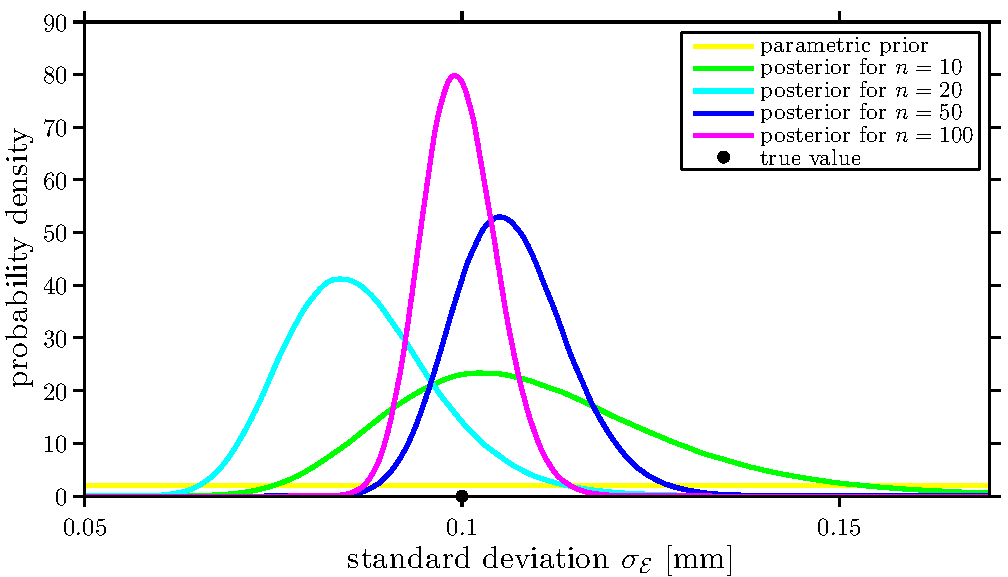
\includegraphics[height=\PEMfigHeight]{fig_PEM_ResCalPostResidualSigma}
    \captionof{figure}[Posterior marginals of \(\sigma_{\mathcal{E}}\)]{Posterior marginals of \(\sigma_{\mathcal{E}}\).
    The marginal posterior of \(\sigma_{\mathcal{E}}\) is shown for different numbers of data \(n\).
    }
    \label{fig:PEM:ResCal:Post:Mean}
  \end{minipage}%
  \hfill%
  % TABLE: RESIDUAL CALIBRATION
  \begin{minipage}[c]{0.46\textwidth}
    \captionof{table}[Summary of the \(\sigma_{\mathcal{E}}\)-marginals]{Summary of the \(\sigma_{\mathcal{E}}\)-marginals.}
    \label{tab:PEM:ResCal:Summary}
    \centering
    \begin{tabular}{lrrrrr}
      \toprule
      & \phantom{} & \multicolumn{3}{c}{\(\sigma_{\mathcal{E}}\) \(\lbrack\unit[10^{-5}]{m}\rbrack\)} & \multicolumn{1}{c}{\(\lbrack \unitless \rbrack\)} \\
      \cmidrule{3-6}
      && \multicolumn{1}{c}{Mean} & \multicolumn{1}{c}{Mode} & \multicolumn{1}{c}{SD} & \multicolumn{1}{c}{CV} \\
      \midrule
      \(n=10\)  && \(11.00\) & \(10.23\) & \(1.90\) & \(0.17\) \\
      \(n=20\)  && \(8.68\)  & \(8.38\)  & \(1.01\) & \(0.12\) \\
      \(n=50\)  && \(10.65\) & \(10.50\) & \(0.77\) & \(0.07\) \\
      \(n=100\) && \(9.97\)  & \(9.90\)  & \(0.50\) & \(0.05\) \\
      \bottomrule
    \end{tabular}
  \end{minipage}%
\end{figure}